\documentclass[11pt,a4paper]{article}

\usepackage[a4paper,top=2.5cm,bottom=2.5cm,left=2cm,right=2cm]{geometry}
\usepackage[T1]{fontenc}
\usepackage{newtxtext}
\usepackage{amsmath,amssymb}
\usepackage{xcolor}
\usepackage{enumitem}
\usepackage{titlesec}
\usepackage{graphicx}
\usepackage{float}
\usepackage{booktabs}
\usepackage{tabularx}
\usepackage{array}
\usepackage{hyperref}
\hypersetup{colorlinks=true,linkcolor=blue,citecolor=blue,urlcolor=blue}

\definecolor{commentgray}{RGB}{90,90,90}
\definecolor{locationblue}{RGB}{22,73,140}
\newenvironment{reviewercomment}{\begin{quote}\small\itshape\color{commentgray}}{\end{quote}}
\newcommand{\authorresponse}{\noindent\textbf{Response:}\quad}
\newcommand{\revisionlocation}[1]{\par\noindent\textcolor{locationblue}{\textbf{Location in the revised manuscript: }}#1}
\newcommand{\draftplaceholder}[1]{\textcolor{red}{\textbf{[PENDING: #1]}}}
\titleformat{\section}{\large\bfseries}{}{0pt}{}
\titleformat{\subsection}{\normalsize\bfseries}{}{0pt}{}
\setlength{\parindent}{0pt}
\setlength{\parskip}{0.45em}

\begin{document}

\begin{center}
{\LARGE\textbf{Response Letter}}\\[1em]
\textbf{Manuscript number:} NETJOURNAL-D-26-00829\\
\textbf{Revised title:}\parbox[t]{0.82\textwidth}{\centering A deep-learning method based on the variable-domain integral weak-solution formulation for neutron diffusion equations with piecewise material coefficients}\\[0.5em]
\textbf{Journal:} Nuclear Engineering and Technology\\[0.5em]
% AUTOFILL:EN_STATUS:BEGIN
\textbf{Current package status:}\textcolor{red}{\texttt{draft\_with\_placeholders}}
% AUTOFILL:EN_STATUS:END
\end{center}

\vspace{1em}
Dear Editor and Reviewers,

% AUTOFILL:EN_INTRO:BEGIN
We sincerely thank the editor and both reviewers for their careful and constructive evaluation. We have repositioned the contribution, rewritten the abstract, expanded the mathematical and implementation details of VIWS, and clarified the networks, loss functions, optimization, sampling, and joint eigenvalue solution. We have also added axial-average results for the three-dimensional rod-bundle case, inference-only PINN--VIWS measurements for the 2D and 3D cases, and a resolution-dependent memory benchmark for the 2D-IAEA case. The matched three-run PINN--VIWS training comparison is not yet complete. Its error and training-time locations remain visibly marked, and no values will be inserted before the corresponding server logs are generated and verified.
% AUTOFILL:EN_INTRO:END

The reviewer comments are reproduced below, followed by our point-by-point responses and manuscript locations.

\section*{Response to Reviewer \#1}

\subsection*{R1.P -- Reviewer overview}
\begin{reviewercomment}
This paper proposes a deep learning framework for solving neutron diffusion equations in heterogeneous media. The primary challenge addressed is the presence of discontinuous diffusion coefficients and macroscopic cross sections at material interfaces. These discontinuities introduce flux-gradient jumps and interface singularities that may adversely affect the accuracy and convergence of neural-network-based solvers. To address this issue, the authors formulate the neutron diffusion equation using a Variable-Domain Integral Weak Solution (VIWS) approach and employ a single-network representation of the global solution. The proposed methodology aims to solve heterogeneous neutron diffusion problems without requiring explicit treatment of internal material interfaces. The topic is relevant and potentially valuable for the application of deep learning methods in reactor physics. However, the manuscript lacks sufficient methodological and implementation details to allow readers to fully understand, reproduce, and evaluate the proposed approach. The following comments should be addressed.
\end{reviewercomment}
% AUTOFILL:EN_R1P:BEGIN
\authorresponse We thank the reviewer for these comments. In response, we have made the VIWS mathematical formulation and its embedding in standard fully connected networks explicit, added the complete loss and training algorithm, clarified all network inputs, outputs, and roles, and expanded the numerical evidence and limitations. The still-pending matched training-cost results remain visibly marked and will not be filled without verified logs.
% AUTOFILL:EN_R1P:END
The corresponding change appears on page \draftplaceholder{page no.} (line \draftplaceholder{line no.}).
\revisionlocation{Title, Abstract, Sections 3.3--3.4 and 4, and the Conclusion.}

\subsection*{R1.1 -- Comment 1}
\begin{reviewercomment}
The abstract does not clearly identify the comparison baseline. It would be beneficial to explicitly state whether the proposed method is compared against conventional PINNs, finite element methods (FEM), finite difference methods (FDM), or other established neutron diffusion solvers. In addition, the abstract does not provide any indication of computational cost, training time, memory requirements, or scalability to large-scale reactor calculations.
\end{reviewercomment}
% AUTOFILL:EN_R11:BEGIN
\authorresponse We thank the reviewer for these comments. We have completely rewritten the abstract and now distinguish the two baselines. FEM provides high-accuracy reference solutions, while the standard PINN is the quantitative neural baseline. The revised abstract reports representative errors for the 2D hexagonal, 3D eight-region, and 2D-IAEA cases. We added inference-only measurements for the common PINN/VIWS flux architecture at 10,000 and 216,000 coordinates, and measured inference time and peak GPU memory for $100^2$--$800^2$ 2D-IAEA query grids. The matched three-run 2D and 3D training errors and training times remain pending, so we retain visible placeholders and do not claim that VIWS is faster than conventional solvers.
% AUTOFILL:EN_R11:END
The corresponding change appears on page \draftplaceholder{page no.} (line \draftplaceholder{line no.}).
\revisionlocation{Abstract; opening of Section 4; matched-cost table; 2D-IAEA inference-memory table.}

\subsection*{R1.2 -- Comment 2}
\begin{reviewercomment}
The manuscript should provide a more detailed discussion regarding the existence and uniqueness conditions associated with the antiderivative formulation employed in the proposed methodology.
\end{reviewercomment}
\authorresponse We thank the reviewer for these comments. The revised manuscript constructs an antiderivative of a continuous kernel by repeated integration with fixed lower limits, which establishes existence. We then explain that the mixed-derivative relation alone is nonunique. Following the cited VIWS theory, we select a representative in an affine correction family. Three noncollinear points determine the correction in 2D, and four noncoplanar points determine it in 3D. We explicitly limit the uniqueness statement to this affine family. Discontinuous reaction kernels are evaluated by segmented regional quadrature rather than by a forced global antiderivative. The corresponding change appears on page \draftplaceholder{page no.} (line \draftplaceholder{line no.}).
\revisionlocation{Section 3.3, “Antiderivative transformation,” including the affine-family equation and its discussion.}

\subsection*{R1.A -- Unnumbered architecture comment}
\begin{reviewercomment}
The neural-network architecture is insufficiently described. If separate antiderivative and neutron-flux networks are employed, their structures should be explicitly specified. At a minimum, the following information should be provided:
\begin{enumerate}[label=\alph*.,leftmargin=2em]
\item Network structure
\item Number of hidden layers
\item Number of neurons per layer
\item Activation functions
\item Input/output variables
\item Training strategy
\end{enumerate}
\end{reviewercomment}
\authorresponse We thank the reviewer for these comments. We now provide the complete architecture and training description. Each energy group has one global flux network over the full domain. Each flux network has eight hidden layers with 32 neurons per layer, and each antiderivative network has six hidden layers with 32 neurons per layer. All use Tanh activations, and the hidden-layer counts exclude the input and output layers. The networks receive 2D or 3D spatial coordinates and return scalar fields. Training uses Adam followed by L-BFGS.

For clarity, the key implementation choices added to the revised manuscript are summarized below.

\begin{table}[H]
\centering
\small
\caption{Key network roles and training choices added to the revised manuscript.}
\label{tab:response_network_settings}
\renewcommand{\arraystretch}{1.15}
\begin{tabularx}{0.98\textwidth}{@{}p{2.7cm}p{2.6cm}p{2.4cm}X@{}}
\toprule
Component & Input / output & Architecture & Role and training \\
\midrule
Flux network & Spatial coordinates / scalar flux & 8 hidden layers $\times$ 32, Tanh & One global network per energy group; optimized with Adam followed by L-BFGS. \\
Antiderivative network & Spatial coordinates / scalar auxiliary field $F_k$ & 6 hidden layers $\times$ 32, Tanh & Represents continuous VIWS kernels in the fixed-source cases and is optimized jointly with the flux network. \\
Eigenvalue implementation & Coordinates / two scalar group fluxes; global $k_{\mathrm{eff}}$ & Two 8 $\times$ 32 flux networks & The two flux networks and $k_{\mathrm{eff}}$ are jointly optimized; the structured-grid IAEA case uses direct cumulative quadrature. \\
\bottomrule
\end{tabularx}
\end{table}
The corresponding change appears on page \draftplaceholder{page no.} (line \draftplaceholder{line no.}).
\revisionlocation{Section 3.4 and the network/optimization settings table.}

\subsection*{R1.3 -- Comment 3}
\begin{reviewercomment}
The optimization procedure is not adequately described. The manuscript should clearly state the trainable parameters, optimization algorithm(s), learning-rate strategy, and any additional optimization settings used during training.
\end{reviewercomment}
\authorresponse We thank the reviewer for these comments. We now state that the trainable variables are the flux-network parameters, antiderivative-network parameters, and the global scalar $k_{\mathrm{eff}}$ for eigenvalue problems. Adam runs for 2,000 iterations with an initial learning rate of $10^{-3}$, followed by L-BFGS. The L-BFGS iteration cap, history size, tolerances, and strong-Wolfe line search are listed in one settings table. Loss weights and Fourier matrices are fixed. A neural test function, when required, is pretrained and then frozen. The corresponding change appears on page \draftplaceholder{page no.} (line \draftplaceholder{line no.}).
\revisionlocation{Section 3.4, the training algorithm, and the network/optimization settings table.}

\subsection*{R1.4 -- Comment 4}
\begin{reviewercomment}
The manuscript states that training terminates when the loss reaches a prescribed accuracy requirement or satisfies a stopping criterion. However, neither the accuracy requirement nor the stopping criterion is explicitly defined. Since References 38 and 39 are cited for these details, and one of these references is not readily accessible to an international audience, the relevant information should be included directly in the manuscript.
\end{reviewercomment}
% AUTOFILL:EN_R14:BEGIN
\authorresponse We thank the reviewer for these comments. We deleted the undefined phrase “preset accuracy requirement.” Adam stops after 2,000 iterations. L-BFGS stops at its maximum iteration count, gradient tolerance, or parameter/objective-change tolerance. These rules are now stated directly in the manuscript. \draftplaceholder{Insert the actual stopping iteration and final loss after the matched reruns are completed.}
% AUTOFILL:EN_R14:END
The corresponding change appears on page \draftplaceholder{page no.} (line \draftplaceholder{line no.}).
\revisionlocation{Section 3.4 and the network/optimization settings table.}

\subsection*{R1.5 -- Comment 5}
\begin{reviewercomment}
The term L-BFGS appears in Section 4 without prior introduction. The authors should provide the full name and briefly explain its role within the optimization procedure.
\end{reviewercomment}
\authorresponse We thank the reviewer for these comments. At first use, we now write “limited-memory Broyden--Fletcher--Goldfarb--Shanno (L-BFGS) algorithm.” We explain that it provides limited-memory quasi-Newton refinement after Adam obtains a stable initialization. We do not make a global-convergence claim. The corresponding change appears on page \draftplaceholder{page no.} (line \draftplaceholder{line no.}).
\revisionlocation{Section 3.4, optimization paragraph.}

\subsection*{R1.6 -- Comment 6}
\begin{reviewercomment}
The manuscript states that the ``default network is an 8-layer FCNN.'' The meaning of ``default'' should be clarified. Is this architecture used throughout all numerical experiments, or only when otherwise unspecified?
\end{reviewercomment}
\authorresponse We thank the reviewer for these comments. We removed “default network” and replaced it with an explicit common architecture for the reported experiments. We also clarify that hidden-layer counts exclude the input and output layers. The corresponding change appears on page \draftplaceholder{page no.} (line \draftplaceholder{line no.}).
\revisionlocation{Section 3.4, the settings table, and the opening of Section 4.}

\subsection*{R1.7 -- Comment 7}
\begin{reviewercomment}
The manuscript should explicitly state the number and physical meaning of the input and output variables used by each neural network.
\end{reviewercomment}
\authorresponse We thank the reviewer for these comments. The flux networks receive only $(x,y)$ or $(x,y,z)$ and return one scalar flux per energy group. Each antiderivative network receives the same coordinates and returns one scalar auxiliary field. Material data and sources are queried by coordinate and enter the residual, but they are not network inputs. Fourier features are a fixed coordinate map. The scalar $k_{\mathrm{eff}}$ is optimized globally and is neither a spatial-network input nor output. The corresponding change appears on page \draftplaceholder{page no.} (line \draftplaceholder{line no.}).
\revisionlocation{Section 3.4, immediately after the flux- and antiderivative-network definitions.}

\subsection*{R1.8 -- Comment 8}
\begin{reviewercomment}
The incorporation of the VIWS formulation into the deep learning framework is not sufficiently explained. It is important to clearly identify where the VIWS formulation enters the neural-network training process and how it contributes to the loss function or governing constraints.
\end{reviewercomment}
\authorresponse We thank the reviewer for these comments. We added explicit definitions of the VIWS residual loss $\mathcal L_{\mathrm r}$, antiderivative definition loss $\mathcal L_{\mathrm{def}}$, determining-point loss $\mathcal L_F$, boundary loss $\mathcal L_{\mathrm b}$, and eigenvalue normalization loss $\mathcal L_{\mathrm{norm}}$. The new pseudocode traces sampling, flux and derivative evaluation, kernel construction, segmented integration, loss assembly, and joint optimization. The corresponding change appears on page \draftplaceholder{page no.} (line \draftplaceholder{line no.}).
\revisionlocation{Section 3.4, the loss equations and the VIWS training algorithm.}

\subsection*{R1.9 -- Comment 9}
\begin{reviewercomment}
It is not entirely clear whether the neutron diffusion equation is enforced through integral residuals derived from the VIWS formulation or through an alternative implementation. This aspect should be clarified.
\end{reviewercomment}
\authorresponse We thank the reviewer for these comments. The governing equation is enforced by the VIWS variable-domain integral residual, not by the original strong-form residual. Continuous diffusion and boundary kernels use antiderivative networks and automatic differentiation. Absorption, scattering, fission, and source terms with piecewise material data use segmented regional quadrature. No explicit internal-interface penalty is added. The corresponding change appears on page \draftplaceholder{page no.} (line \draftplaceholder{line no.}).
\revisionlocation{Sections 3.3--3.4, including the implementation paragraph following the total loss.}

\subsection*{R1.10 -- Comment 10}
\begin{reviewercomment}
Statements such as ``antiderivative forms are used in the deep learning solution'' are difficult for readers to interpret. The manuscript would benefit from a more explicit explanation of how the antiderivative formulation is incorporated into the training procedure and how it contributes to computational efficiency.
\end{reviewercomment}
\authorresponse We thank the reviewer for these comments. We now explain that mixed derivatives of the auxiliary networks reconstruct continuous kernels through $\mathcal L_{\mathrm{def}}$, while the auxiliary values enter the VIWS residual $\mathcal L_{\mathrm r}$. This can reduce repeated cumulative quadrature of continuous kernels but adds auxiliary-network and automatic-differentiation costs. We therefore removed unconditional efficiency claims and do not attribute the overall VIWS--PINN timing to one component. The corresponding change appears on page \draftplaceholder{page no.} (line \draftplaceholder{line no.}).
\revisionlocation{Sections 3.3--3.4 and the limitations paragraph in the Conclusion.}

\subsection*{R1.11 -- Comment 11}
\begin{reviewercomment}
I think the paper is not proposing a new neural network architecture. Rather, it is proposing a new mathematical formulation (VIWS) that is embedded into a deep-learning framework to better handle material interfaces in heterogeneous neutron diffusion problems. If so, please include this explicitly in your manuscript.
\end{reviewercomment}
\authorresponse We thank the reviewer for these comments. We fully agree. The title, abstract, introduction, Methods, and Conclusion now state that the contribution is the VIWS mathematical governing formulation and its implementation in standard fully connected networks, rather than a new neural-network architecture. The corresponding change appears on page \draftplaceholder{page no.} (line \draftplaceholder{line no.}).
\revisionlocation{Title; Abstract; end of the Introduction; opening of Section 3.4; Conclusion.}

\subsection*{R1.12 -- Comment 12}
\begin{reviewercomment}
How do the execution time and memory compare against conventional NDE solvers?
\end{reviewercomment}
% AUTOFILL:EN_R112:BEGIN
\authorresponse We thank the reviewer for these comments. The revised manuscript limits quantitative cost comparisons to matched standard PINN and VIWS implementations. FEM remains the high-accuracy reference and is discussed qualitatively. Inference-only tests of the common eight-hidden-layer flux network are now complete: the 2D tests use 10,000 coordinates and require 0.00217~s for PINN and 0.00208~s for VIWS, with 14.221~MiB peak GPU memory; the 3D tests use 216,000 coordinates and require 0.03914~s and 0.03953~s, with 119.598~MiB peak memory. These are deployment-time measurements, not training-memory claims. Because we have not established a same-platform, same-tolerance comparison with a mature NDE solver, we explicitly state that this work does not demonstrate a speed advantage over conventional solvers. \draftplaceholder{Insert the matched three-run 2D and 3D relative-error and training-time data from the server runs.}
% AUTOFILL:EN_R112:END

The most relevant matched cost quantities are shown directly here so that the revision can be checked without searching through the manuscript. The red entries remain deliberately unresolved until the twelve server runs have been completed and verified.

\begin{table}[H]
\centering
\caption{Matched PINN--VIWS accuracy and cost comparison reported in the revised manuscript. Values are medians [ranges] over three runs.}
\label{tab:response_matched_cost}
\renewcommand{\arraystretch}{1.15}
\resizebox{\textwidth}{!}{%
\begin{tabular}{@{}llcccc@{}}
\toprule
Case & Method & Relative $L_2$ error & Training time & Inference time (s) & Peak GPU memory (MiB) \\
\midrule
% AUTOFILL:EN_MATCHED_TABLE:BEGIN
2D hexagon & PINN & \textcolor{red}{TBD} & \textcolor{red}{TBD} & 0.00217 [0.00213, 0.00223] & 14.221 [14.221,14.221] \\
2D hexagon & VIWS & \textcolor{red}{TBD} & \textcolor{red}{TBD} & 0.00208 [0.00207, 0.00208] & 14.221 [14.221,14.221] \\
3D eight-region & PINN & \textcolor{red}{TBD} & \textcolor{red}{TBD} & 0.03914 [0.03905, 0.03926] & 119.598 [119.598,119.598] \\
3D eight-region & VIWS & \textcolor{red}{TBD} & \textcolor{red}{TBD} & 0.03953 [0.03833, 0.03982] & 119.598 [119.598,119.598] \\
% AUTOFILL:EN_MATCHED_TABLE:END
\bottomrule
\end{tabular}}
\end{table}
The corresponding change appears on page \draftplaceholder{page no.} (line \draftplaceholder{line no.}).
\revisionlocation{End of the Abstract; opening of Section 4; matched-cost table; Conclusion.}

\section*{Response to Reviewer \#2}

\subsection*{R2.G1 -- General Comment 1}
\begin{reviewercomment}
The title of the manuscript is a bit misleading. What exactly is ``heterogeneous neutron diffusion calculations''? If the method requires any cross-material homogenization (for example, each pin cell is homogenized, so there are no separate cladding, air gap, fuel and moderator cells), then the word ``heterogeneous'' is not applicable to the manuscript and should be changed to a more appropriate term.
\end{reviewercomment}
\authorresponse We thank the reviewer for these comments. We changed the title to “A deep-learning method based on the variable-domain integral weak-solution formulation for neutron diffusion equations with piecewise material coefficients.” The 2D hexagonal case explicitly distinguishes fuel, cladding, and moderator regions. The 3D rod case distinguishes rods and the exterior material. The 2D-IAEA case uses assembly-homogenized two-group constants. We now use “piecewise-defined material coefficients” whenever that term is more precise than “heterogeneous.” The corresponding change appears on page \draftplaceholder{page no.} (line \draftplaceholder{line no.}).
\revisionlocation{Title; Abstract; Introduction; model-scale description in Section 4.5.}

\subsection*{R2.G2 -- General Comment 2}
\begin{reviewercomment}
The quality of the abstract is much lower than the quality of the main body of the manuscript. While the manuscript itself is concise, uses correct terminology and is overall understandable, the abstract does a poor job representing the manuscript. Some sentences in the abstract make no sense at all, so the authors are required to completely rewrite the abstract and carefully proofread it to match the quality of the manuscript's main body.
\end{reviewercomment}
\authorresponse We thank the reviewer for these comments. We accepted this comment and completely rewrote the abstract. It now presents the piecewise-parameter problem, the standard-PINN difficulty, the VIWS formulation, the separate treatment of continuous and discontinuous kernels, the FEM and PINN baselines, quantitative 2D/3D/IAEA results, computational cost, and the scope boundary. The corresponding change appears on page \draftplaceholder{page no.} (line \draftplaceholder{line no.}).
\revisionlocation{Entire Abstract.}

\subsection*{R2.G3 -- General Comment 3}
\begin{reviewercomment}
An important aspect of introducing PINNs in place of traditional neutron diffusion solvers is their potential advantage in computational speed. How does the proposed method compare -- apples-to-apples (using exactly the same number of CPU cores/GPU cards, the same models) -- to conventional solvers, and if it is faster, what are the accuracy trade-offs that we can expect? What about memory consumption?
\end{reviewercomment}
% AUTOFILL:EN_R2G3:BEGIN
\authorresponse We thank the reviewer for these comments. We agree that cross-hardware, cross-implementation, or cross-tolerance timings are not an apples-to-apples comparison. Quantitative cost reporting is therefore limited to matched standard PINN and VIWS settings, and FEM is used as the accuracy reference. The 2D and 3D inference-only tests now report the measured time and peak GPU memory of the common final flux architecture, while the 2D-IAEA resolution study reports inference time, peak GPU memory, output memory, and model memory. We do not claim that VIWS is faster than conventional solvers. \draftplaceholder{Insert the matched three-run 2D and 3D relative-error and training-time results from the server runs.}
% AUTOFILL:EN_R2G3:END
The corresponding change appears on page \draftplaceholder{page no.} (line \draftplaceholder{line no.}).
\revisionlocation{Abstract; opening of Section 4; matched-cost and 2D-IAEA memory tables; Conclusion.}

\subsection*{R2.G4 -- General Comment 4}
\begin{reviewercomment}
While the presented method seems to be of high value, the potential disadvantages of the method were not clearly stated, so the manuscript reads more like an advertisement, whereas a scientific paper should present both positives and negatives of the work that were observed.
\end{reviewercomment}
\authorresponse We thank the reviewer for these comments. We rewrote the Conclusion and added a substantive limitations paragraph. It addresses per-problem nonconvex retraining, sensitivity to sampling and optimization, auxiliary-network and automatic-differentiation costs, segmented quadrature for discontinuous reaction kernels, geometry and test-function construction, the present validation scale, untested boundary types, the lack of a production-solver benchmark, and the absence of a general posterior error or convergence guarantee. Promotional and unsupported efficiency language was removed throughout. The corresponding change appears on page \draftplaceholder{page no.} (line \draftplaceholder{line no.}).
\revisionlocation{Third paragraph of the Conclusion and related claim softening in the Abstract and Section 4.}

\subsection*{R2.G5 -- General Comment 5}
\begin{reviewercomment}
The proposed method could be introduced in a more reproducible way, which was not the case in the submitted manuscript. The reader will need to dig through all the literature sources mentioned and beyond to piece together the exact pathway on how to implement a similar solver. The manuscript would greatly benefit from having a more straightforward algorithm that the authors used to create the model, train it, and then use in practice. The authors are kindly reminded that they submit their work to the journal named ``Nuclear Engineering and Technology'', and while ``Nuclear'' is clearly present in the manuscript, there is no ``Engineering'' and/or ``Technology'' presented. This makes it look more like a scientific report than an original article. The authors are requested to close this gap.
\end{reviewercomment}
\authorresponse We thank the reviewer for these comments. The method section is now self-contained. It specifies the network inputs and outputs, five loss terms, continuous/discontinuous evaluation paths, training pseudocode, common network architecture, optimization parameters, and stopping rules. Engineering relevance is made concrete through the 177-location assembly-homogenized 2D-IAEA benchmark, its two-group fluxes, 22 pcm eigenvalue deviation, and measured resolution-dependent resource cost. The manuscript does not rely on an unavailable code repository to explain the implementation, and we make no code-release claim. The corresponding change appears on page \draftplaceholder{page no.} (line \draftplaceholder{line no.}).
\revisionlocation{Sections 3.3--3.4, training algorithm and settings table, and Section 4.5.}

\subsection*{R2.S1 -- Specific Comment 1: Abstract}
\begin{reviewercomment}
``Neutron diffusion calculations are essential in reactor physics, but heterogeneous reactor cores contain discontinuous diffusion coefficients and macroscopic cross sections.''

\begin{enumerate}[label=\alph*.,leftmargin=2em]
\item It looks like the authors introduced new and unnecessary terminology in a long-established field. What exactly do the authors mean by ``discontinuous'' diffusion coefficients and ``discontinuous'' macroscopic cross-sections? From the reviewer's view, such combination of words makes no sense.
\item The reviewer is also not convinced that reactor cores contain these coefficients or any other coefficients. The authors are required to proofread the entire Abstract to convey their points in a clearer, more accurate way.
\end{enumerate}
\end{reviewercomment}
\authorresponse We thank the reviewer for these comments. We agree that the original subject and terminology were inaccurate. The sentence now reads: “In multiregion neutron-diffusion models, each material region is represented by its own effective diffusion coefficient and macroscopic cross sections, and these piecewise-defined parameters may change abruptly across material interfaces.” This wording assigns the coefficients to the mathematical model rather than stating that the physical core “contains coefficients.” The corresponding change appears on page \draftplaceholder{page no.} (line \draftplaceholder{line no.}).
\revisionlocation{First sentence of the Abstract and first paragraph of the Introduction.}

\subsection*{R2.S2 -- Specific Comment 2: Fig. 4}
\begin{reviewercomment}
What is antiderivative, and why are antiderivative fields in Fig. 4 not symmetric?
\end{reviewercomment}
\authorresponse We thank the reviewer for these comments. We now define $F$ as a nonphysical auxiliary scalar used to reconstruct an integral kernel. It is not a flux, power, or reaction rate. Its representative depends on the integration directions, test function, and determining points, so its visual symmetry need not match the physical flux. The required condition is that its corresponding mixed derivative reconstructs the target kernel. The revised caption identifies the roles of $F_0$, $F_1$, and $F_2$ and the determining-point condition. The corresponding change appears on page \draftplaceholder{page no.} (line \draftplaceholder{line no.}).
\revisionlocation{Sections 3.3--3.4 and the caption of the 2D hexagonal antiderivative figure.}

\subsection*{R2.S3 -- Specific Comment 3: Section 4.1}
\begin{reviewercomment}
``The total number of interior and boundary sampling points is 10, 000.''

What are the sampling points and how exactly are they used? How is the number determined and why it matters?
\end{reviewercomment}
\authorresponse We thank the reviewer for these comments. We rechecked the implementation and corrected the earlier inaccurate description of 10,000 points as all being interior points. The matched rerun protocol uses a $100\times100$ Cartesian background grid, i.e. 10,000 coordinates before masking; only coordinates inside the hexagon enter the domain losses, and the active count is recorded for every run. It also uses exactly 2,048 boundary points distributed uniformly by arc length over the six edges without duplicated vertices, and three 2D determining points per antiderivative. PINN and VIWS use the identical background grid, domain mask, and boundary points for a given seed, with no interface enrichment. A systematic sampling-density study was not performed and is now stated as a limitation. The corresponding change appears on page \draftplaceholder{page no.} (line \draftplaceholder{line no.}).
\revisionlocation{Sampling paragraph in Section 4.1 and the limitations paragraph in the Conclusion.}

\subsection*{R2.S4 -- Specific Comment 4: Section 4.3}
\begin{reviewercomment}
It would be useful to see axially normalized maps and their comparison. In particular, not only the flux map but also the source map that is calculated by the reference code, PINN, and VIWS.
\end{reviewercomment}
\authorresponse We thank the reviewer for these comments. We added FEM, PINN, and VIWS axial-average flux and total-source maps. The total source is $q_{\mathrm{tot}}=S+\nu\Sigma_{\mathrm f}\phi$. All methods use the corresponding FEM axial-average maximum as the common normalization factor and share color scales. The PINN and VIWS axial-average flux errors are $3.55\times10^{-1}$ and $6.26\times10^{-2}$, respectively. Their total-source errors are $1.00\times10^{-3}$ and $2.28\times10^{-4}$.

The new comparison figure is reproduced below. It shows the FEM, PINN, and VIWS axial-average fields together with the two absolute-error maps for each physical quantity; FEM-based normalization and shared color scales make the comparison direct.

\begin{figure}[H]
\centering
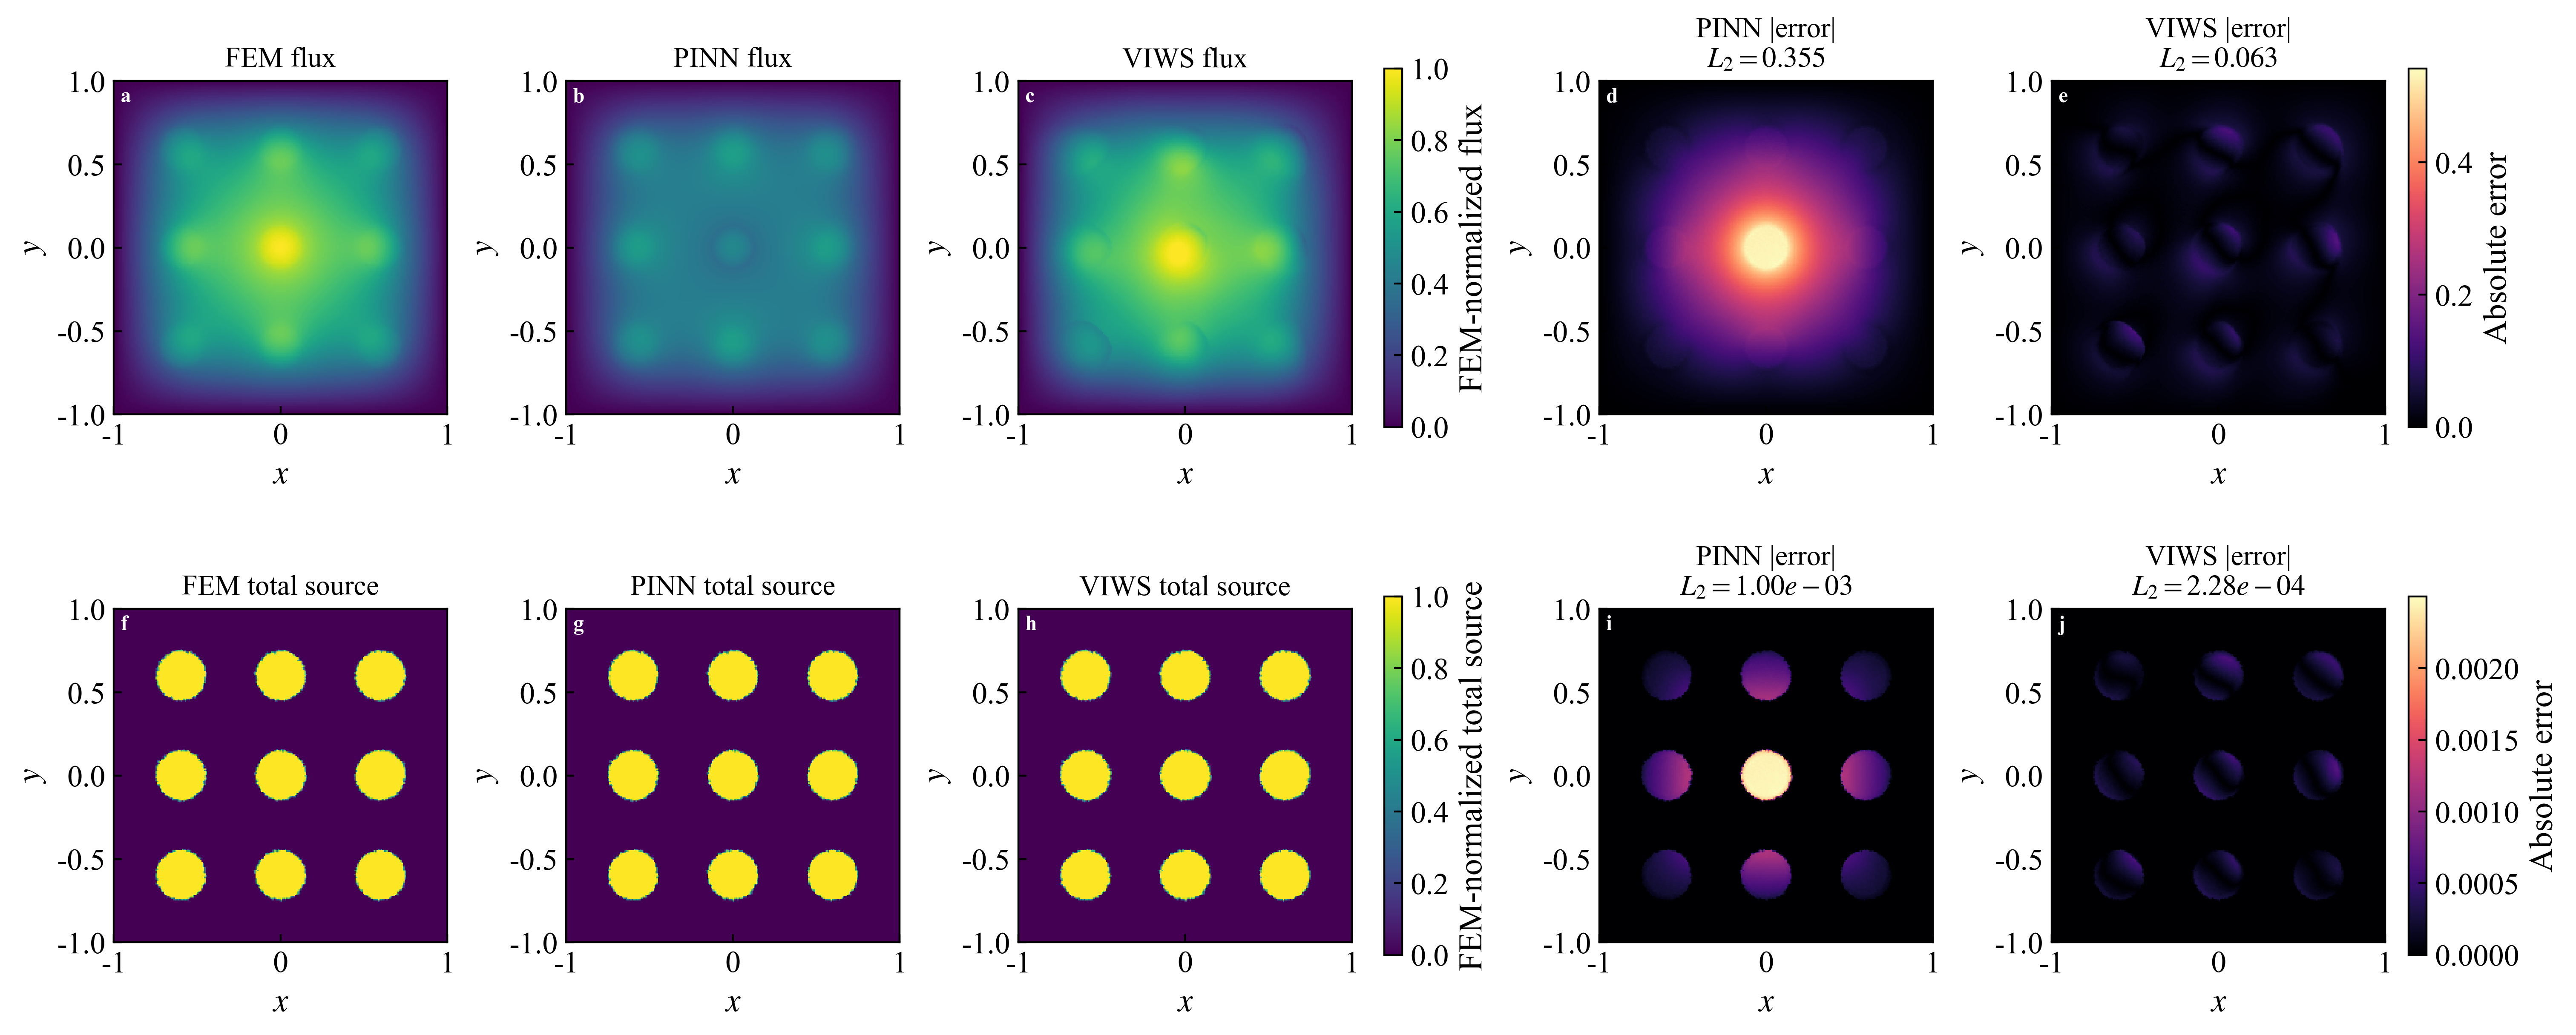
\includegraphics[width=\textwidth]{fig/figure_14.png}
\caption{New axial-average comparison added to the revised manuscript. Panels (a)--(e) show the normalized flux fields and absolute errors; panels (f)--(j) show the normalized total-source fields and absolute errors.}
\label{fig:response_axial_average}
\end{figure}
The corresponding change appears on page \draftplaceholder{page no.} (line \draftplaceholder{line no.}).
\revisionlocation{Section 4.3, axial-average equation and new axial-average comparison figure.}

\subsection*{R2.S5 -- Specific Comment 5: Section 4.4}
\begin{reviewercomment}
What are the limitations of the method in terms of problem size and boundary condition? Can the meshes be of the entire fuel assembly size?
\end{reviewercomment}
\authorresponse We thank the reviewer for these comments. We now distinguish mathematical extensibility from numerical validation. The reported cases verify Dirichlet, Neumann, and mixed boundaries. Robin and periodic boundaries remain untested. The method does not require finite-element connectivity, but it still requires interior, boundary, and determining points. An assembly-homogenized model can be represented by a global coordinate network, but pin-resolved 3D assemblies and full-core models have not been validated and are not claimed. The corresponding change appears on page \draftplaceholder{page no.} (line \draftplaceholder{line no.}).
\revisionlocation{Scope statements in Sections 4.3--4.5 and the limitations paragraph in the Conclusion.}

\subsection*{R2.S6 -- Specific Comment 6: Section 4.5}
\begin{reviewercomment}
``The width of each assembly is 20, cm, and the thickness of the surrounding reflector 290 is also 20, cm.''

\begin{enumerate}[label=\alph*.,leftmargin=2em]
\item Commas before the ``cm'' seem unnecessary.
\item Did the VIMS model output pointwise flux shape, or was there a 2D function per each assembly that could produce the flux shape for each point? Please elaborate on the process of flux output in more detail as well as the memory requirement to produce variable resolution flux.
\item Were the fuel assemblies divided into sub-regions? Also, were the fuel assembly regions homogenized material-wise?
\end{enumerate}
\end{reviewercomment}
\authorresponse We thank the reviewer for these comments. (a) The unit is corrected to $20\,\mathrm{cm}$. (b) The method is VIWS. Each energy group uses one global coordinate-to-flux function over the quarter core, not a separate function per assembly. Model memory is independent of query resolution, whereas coordinates, activations, and output arrays grow with $N_q$, and stored outputs scale as $O(GN_q)$. Double-precision full-grid tests at $100^2$, $200^2$, $400^2$, and $800^2$ give median inference times of 0.00996, 0.03708, 0.10664, and 0.42140 s, with peak GPU memory of 58.379, 207.426, 793.580, and 3,151.043 MiB. (c) The benchmark uses assembly-homogenized two-group constants. Regions $\Omega_1$--$\Omega_4$ represent assembly/reflector material categories and do not resolve fuel, gap, cladding, or moderator subregions.

The measured resolution-resource relation is included below. All entries are from three inference-only repetitions; model memory remains constant while coordinate, activation, and output storage increase with the query grid.

\begin{table}[H]
\centering
\small
\caption{Resolution-dependent full-grid inference cost for the two-group 2D-IAEA case.}
\label{tab:response_iaea_memory}
\renewcommand{\arraystretch}{1.15}
\begin{tabularx}{\textwidth}{@{}lrrrr@{}}
\toprule
Query grid & Query points & Inference time & Peak GPU memory & Output / model memory \\
\midrule
$100^2$ & 10,000 & 0.00996 [0.00992, 0.00998] s & 58.379 MiB & 0.153 / 0.251 MiB \\
$200^2$ & 40,000 & 0.03708 [0.03705, 0.03727] s & 207.426 MiB & 0.610 / 0.251 MiB \\
$400^2$ & 160,000 & 0.10664 [0.10624, 0.11698] s & 793.580 MiB & 2.441 / 0.251 MiB \\
$800^2$ & 640,000 & 0.42140 [0.42136, 0.42252] s & 3,151.043 MiB & 9.766 / 0.251 MiB \\
\bottomrule
\end{tabularx}
\end{table}
The corresponding change appears on page \draftplaceholder{page no.} (line \draftplaceholder{line no.}).
\revisionlocation{Section 4.5, geometry/output/memory paragraphs and the inference-memory table.}

\subsection*{R2.S7 -- Specific Comment 7: Section 4.5}
\begin{reviewercomment}
``The effective multiplication factor $k_{\mathrm{eff}}$ is treated as a global parameter to be optimized and is updated together with the neural network weights [45].''

It would be useful to see the details on how the flux and the multiplication factor were produced within the same VIWS model.
\end{reviewercomment}
\authorresponse We thank the reviewer for these comments. The revised manuscript explains the joint solve. Two global networks represent the fast and thermal fluxes. The independent scalar $k_{\mathrm{eff}}$ is initialized at 1.0 and enters both fission-source residuals through $1/k_{\mathrm{eff}}$. In this structured-grid case with $v=1$, the variable-domain integral residuals are evaluated directly by cumulative numerical quadrature, so no auxiliary antiderivative network is trained. Both flux networks and $k_{\mathrm{eff}}$ are updated jointly by Adam and L-BFGS. A squared fast-group mean-flux normalization constraint fixes the eigenfunction amplitude and excludes the zero solution. The FEM eigenvalue is used only for post-training evaluation, not as supervision. The corresponding change appears on page \draftplaceholder{page no.} (line \draftplaceholder{line no.}).
\revisionlocation{Section 3.4, normalization loss and training algorithm; Section 4.5, normalization equation and joint-optimization paragraph.}

\enlargethispage{3\baselineskip}
\vspace{0.5em}
% AUTOFILL:EN_CLOSING:BEGIN
We again thank the editor and reviewers for their constructive comments. The present package retains explicit placeholders for the pending matched training-cost experiments. We will update the table, abstract, and corresponding responses only after those independent runs have been completed and verified.
% AUTOFILL:EN_CLOSING:END

\begin{flushright}
Sincerely,\\
The Authors
\end{flushright}

\end{document}
